% Chapter 1
% add following line for typesetting from subfiles
% !TeX root = ../uet_thesis.tex
% !TeX root = ../uet_thesis.bbl
% !TeX root = ../references.bib

\chapter{Introduction} % Write in your own chapter title
\label{Chapter1}
\lhead{Chapter 1. \emph{Introduction}} % Write in your own chapter title to set the page header

\section{What Is VLC}
Visible Light Communication (VLC) is a relatively new wireless communication technology that offers a solution to the shortage of wireless spectrum worldwide. It uses visible light rays for information transfer. The core idea behind this technology is the use of fast switching characteristics of now available high efficiency white Light Emitting Diodes (LED) for both illumination as well as wireless data access points. The switching of the light source takes place at a very high frequency that is not perceived by the human eye. Data speeds upto 100Mbps have been demonstrated using commonly available white LEDs  \cite{le2009100}.

\section{A Look From Historical Perspective}
From primitive times man has been using the light signals to convey information. For instance, burning of a fire or diverting sun light using mirrors \cite{webber1875discussion} to inform fellow human beings of impeding danger can be interpreted as crude examples of VLC systems.

As the technology kept on improving so did the capabilities of visible light communication. One form of visible light communication is used by navies around the world to intercommunicate between ships. The ships are equipped with a signalling lamp that is turned on and off to transmit Morse code signals to the neighbouring ships.

%Visible light communicatio from photophone; Graham Bell 
Use of visible light to transmit human voice at longer distances has a long history, dating back to the time of Graham Bell \cite{bell1880photo}. He demonstrated the wireless transmission of human voice by using sun light in year 1880 and named his device a Photophone. It is interesting to note that wireless transmission of human voice using radio waves was invented much later. Photophone modulated the sun beam by a vibrating mirror.  It  changed its shape to converging or diverging mirror according to sound pressure waves. It resulted in intensity modulation of the reflected light beam. A photophone transmitter is shown in figure \ref{fig:photophone_transmitter}

%\texttt{minipage} environment

\begin{figure}[!hbtp]
\centering
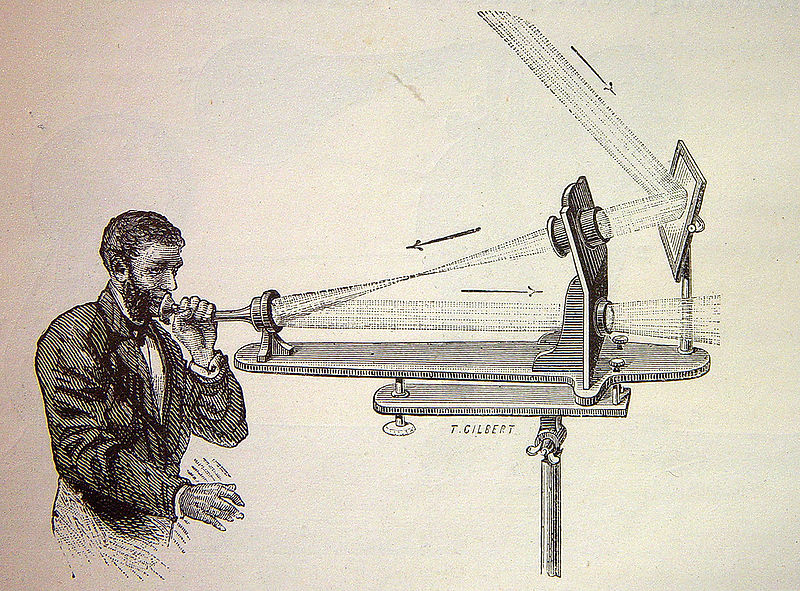
\includegraphics[angle=0,width=\figwidth]{./Figures/Photophone_transmitter.jpg}
\caption[Photophone transmitter]{Graham Bell's photophone transmitter. Sun light modulated with flexible mirror\cite{photoTx}}
%\floatfoot{Source: \url{http://en.wikipedia.org/wiki/File:Photophone_transmitter_4074931746_9f996df841_b.jpg}}
\label{fig:photophone_transmitter}
\end{figure}

%-----------------------------------------------
%\begin{figure}[h]
%%\centering
%\begin{minipage}{.6\textwidth}
%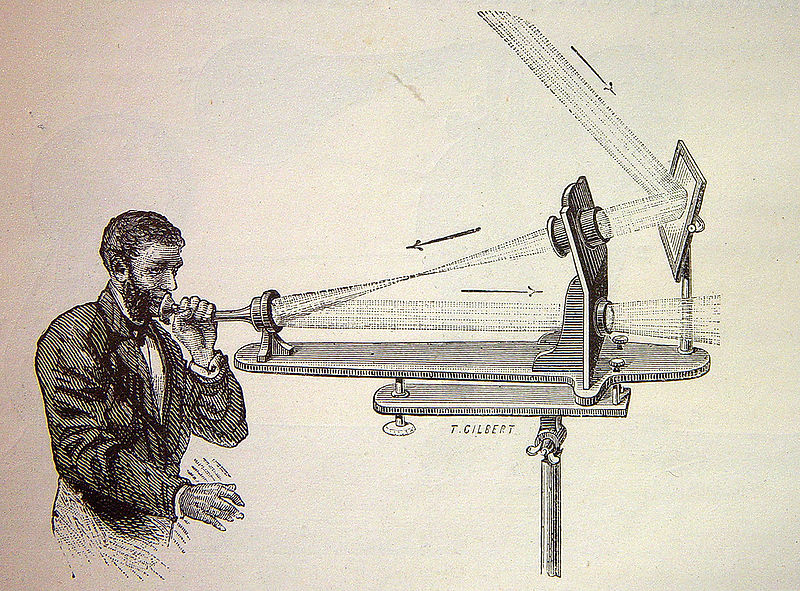
\includegraphics[height=2.9\figheight]{./Figures/Photophone_transmitter.jpg}
%\caption{Lorem}
%\end{minipage}
%\begin{minipage}{.2\textwidth}
%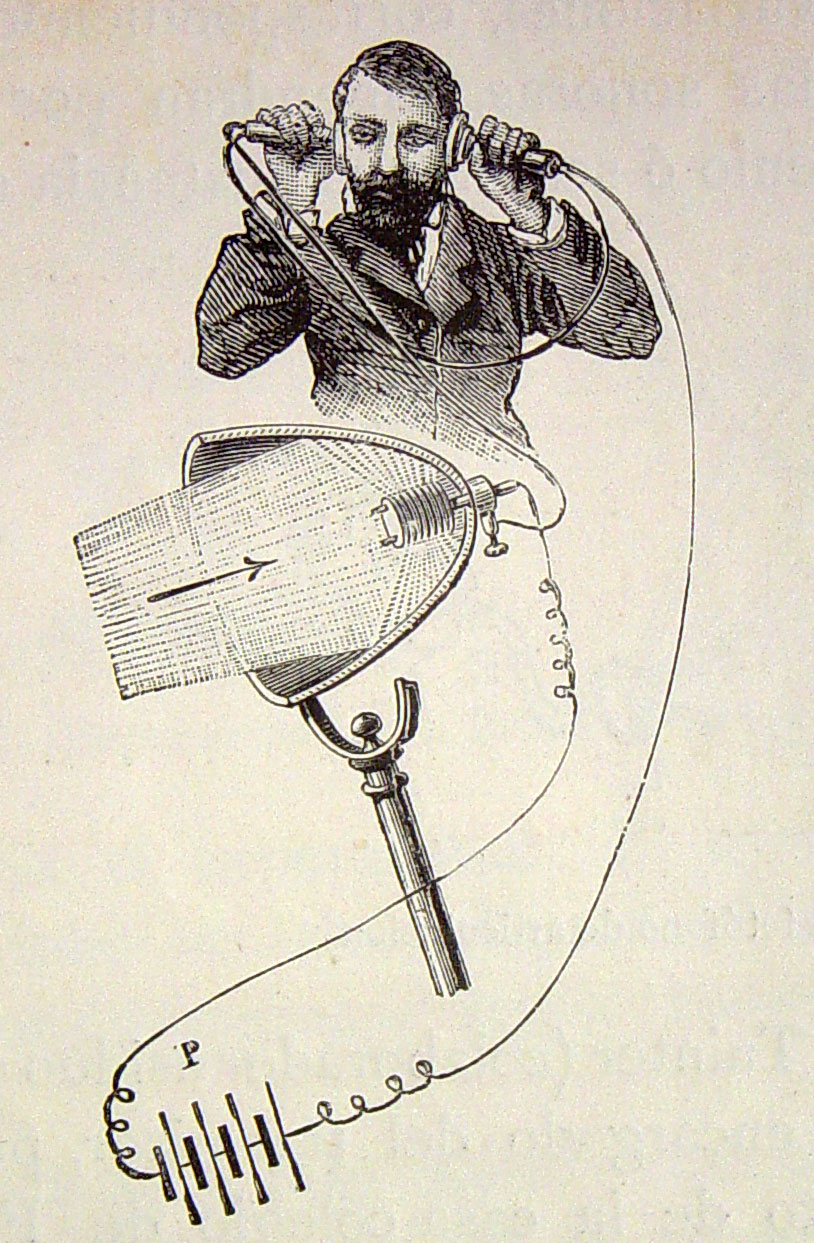
\includegraphics[height=2.9\figheight]{./Figures/Photophone_receiver.jpg}
%\caption{Ipsum}
%\end{minipage}
%\end{figure}
%-----------------------------------------------
%
The receiver consisted of a simpler circuit. It used selenium based crystal detector that conducted electricity in inverse proportion to the incident light. The detector thus converted the incident voice modulated light wave to electric signals. The current passing through detector also energized the speaker coil. The speaker then produced sound according to the current being fed to it. In this way the transmitted voice signal was recovered. The receiver signal is depicted in figure \ref{fig:photophone_receiver}. It is reported that Bell considered photophone his best invention. However it did not enjoy so much popularity as his previous invention of telephone had done. 




\begin{figure}[!hbtp]
\centering
%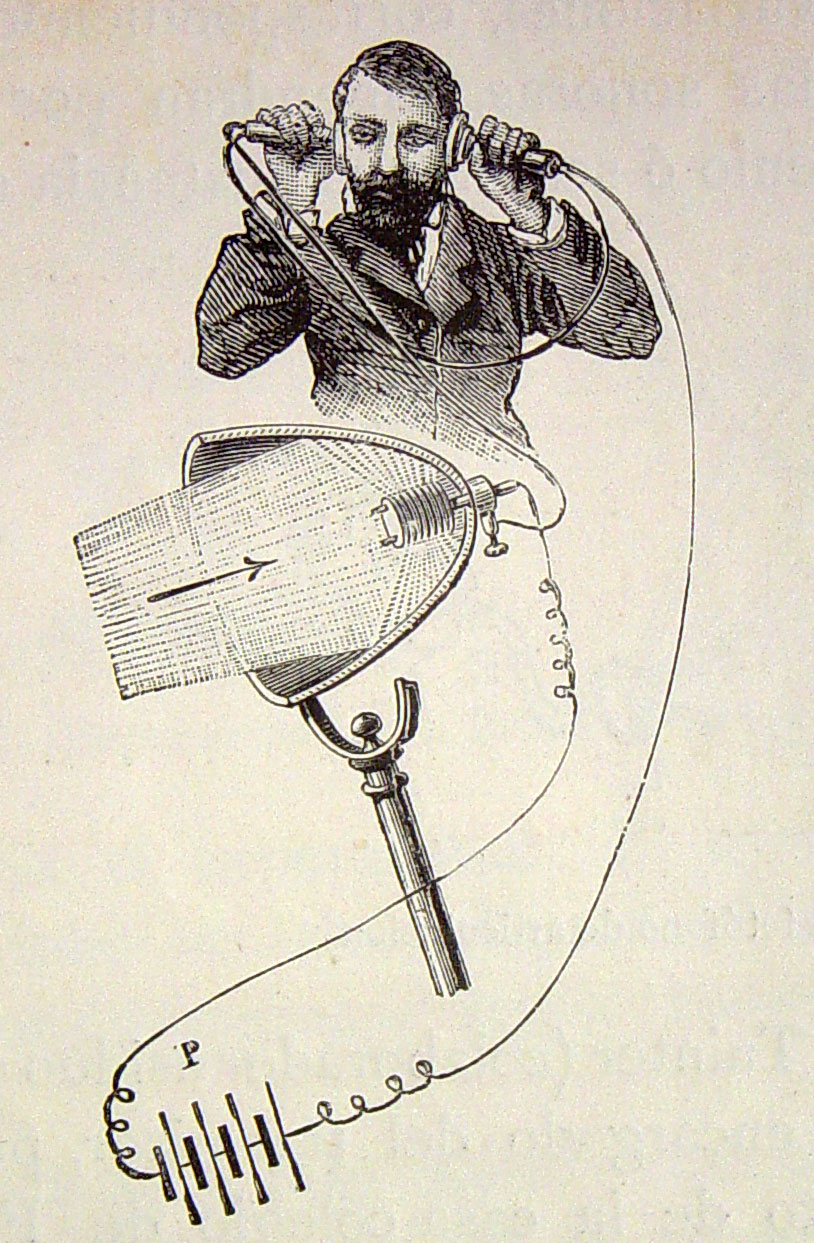
\includegraphics[angle=0,width=\textwidth]{./Figures/Photophone_receiver.jpg}
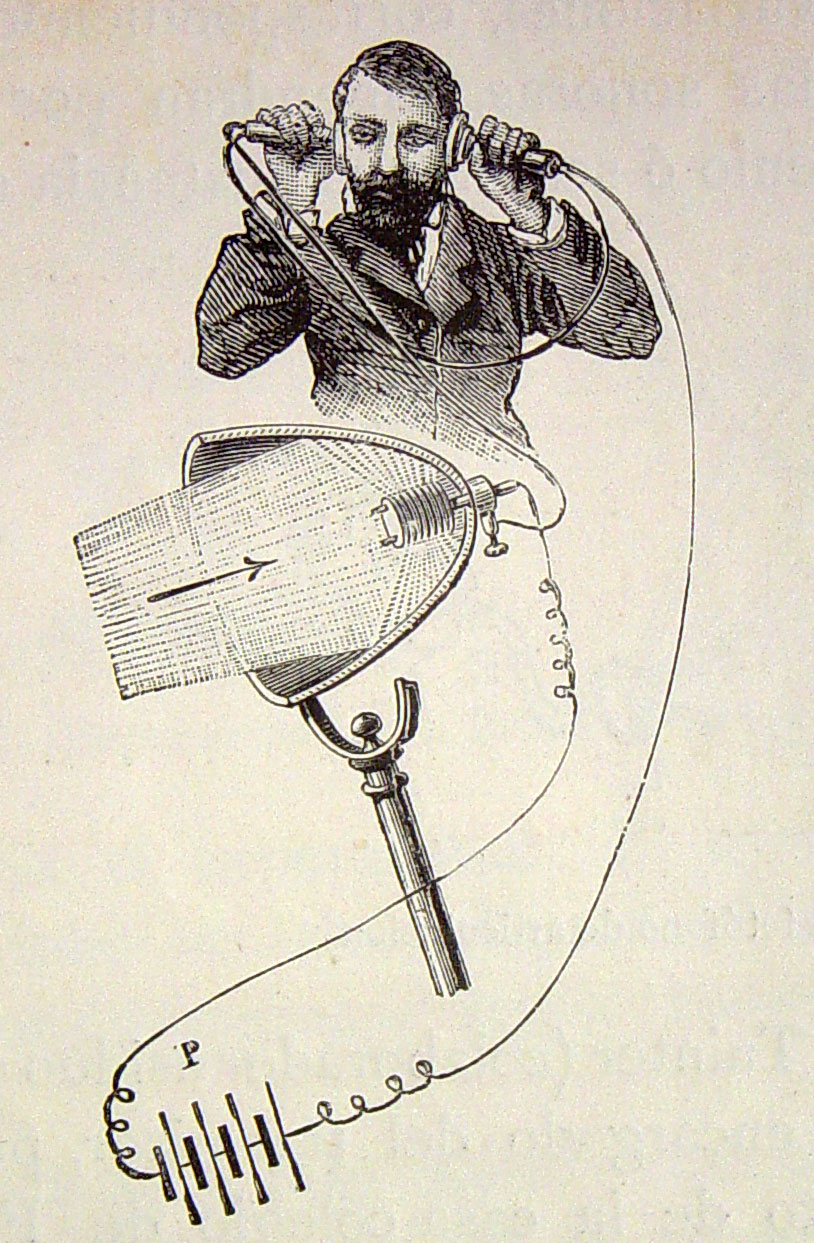
\includegraphics[angle=0,height=7cm]{./Figures/Photophone_receiver.jpg}
\caption[Photophone receiver]{Photophone receiver\cite{photoRx}}
%\floatfoot{Source: \url{http://en.wikipedia.org/wiki/File:Photophone_receiver_4074172975_288f2808f0_o.jpg}}
 \label{fig:photophone_receiver}
\end{figure}
%http://en.wikipedia.org/wiki/File:Photophone_receiver_4074172975_288f2808f0_o.jpg

%-------------------------Complete---------------------------------------------
 

%International consorcium for visibe light communication
%
% What if it could also send streams of data? Traffic lights, television sets, car headlights, billboards and lamps might all suddenly become far more important in our daily lives. We could receive maps from a street light, get news alerts from lamps and download music from electronic posters.


\section{Advantages Of White LEDs Over Conventional Light Sources}



Light emitting diode based solid state lights have gained wide spread popularity in recent years. The active research in high brightness LED electronics has lowered the price with steady improvement in device capabilities. It can be predicted that these solid state devices will be the major illumination source in near future \cite{schubert2005solid}. The LED option is better than conventional filament type Edison light bulbs or gas discharge lamps on several grounds \cite{4781063}. 

%---> Compare LED power efficiency with incadescent and tube lights
%--> Compare LED life expectancy with /////
%\renewcommand{\labelitemi}{$\bullet$}
\begin{list}{$\diamond$}{\setlength{\leftmargin}{.5in}%
\setlength{\rightmargin}{.5in}}

\item Being solid state devices LEDs are capable of switching at frequencies up to several megahertz. This property is very useful to modulate them for high speed data transmission

\item The overall energy efficiency is better than conventional counterparts. An LED can convert up to 80\% of the power intake to the light energy.

\item Light emitting diodes have life expectancy that is several times higher than the competent incandescent type light bulbs, fluorescent tubes and Compact Fluorescent Tubes (CFT).

\item The white light from an RGB (Red-Green-Blue) LED provides control over the hue or light temperature. This feature is quite useful for aesthetics. 

\item Because LEDs are inherently a low voltage and low current device, these can be combined in the form of strings to match for custom voltage and current requirements.

\item LEDs have strong physical structure that makes them suitable in physical vulnerable conditions such as public places or industrial environment.

\item There are lesser environmental hazards associated with the LED lights. Their close counterparts in terms of power efficiency, gas discharge based florescent or compact florescent lamps use mercury that is poisonous to the environment. 

\end{list}

To summarize, LED are a promising choice towards \emph{greener} technology. 

\section{White LED Technology}

White LED are manufactured by using two major distinct device technologies. First one uses the GaInN based blue LED light chip with phosphor encapsulation as shown in figure \ref{fig:phosphor_led}. The blue light emitted from the chip strikes the phosphor that converts the light wavelength from blue to white light. This is the cheaper of the two solution and suffers from two main problems. First of these disadvantages is the requirement of more power as some power is lost in the impact with florescent surface. Secondly the frequency response of phosphor secondary emission is slow that hampers the inherent fast switching characteristics of the LED device.

\begin{figure}[!hbtp]
\centering
%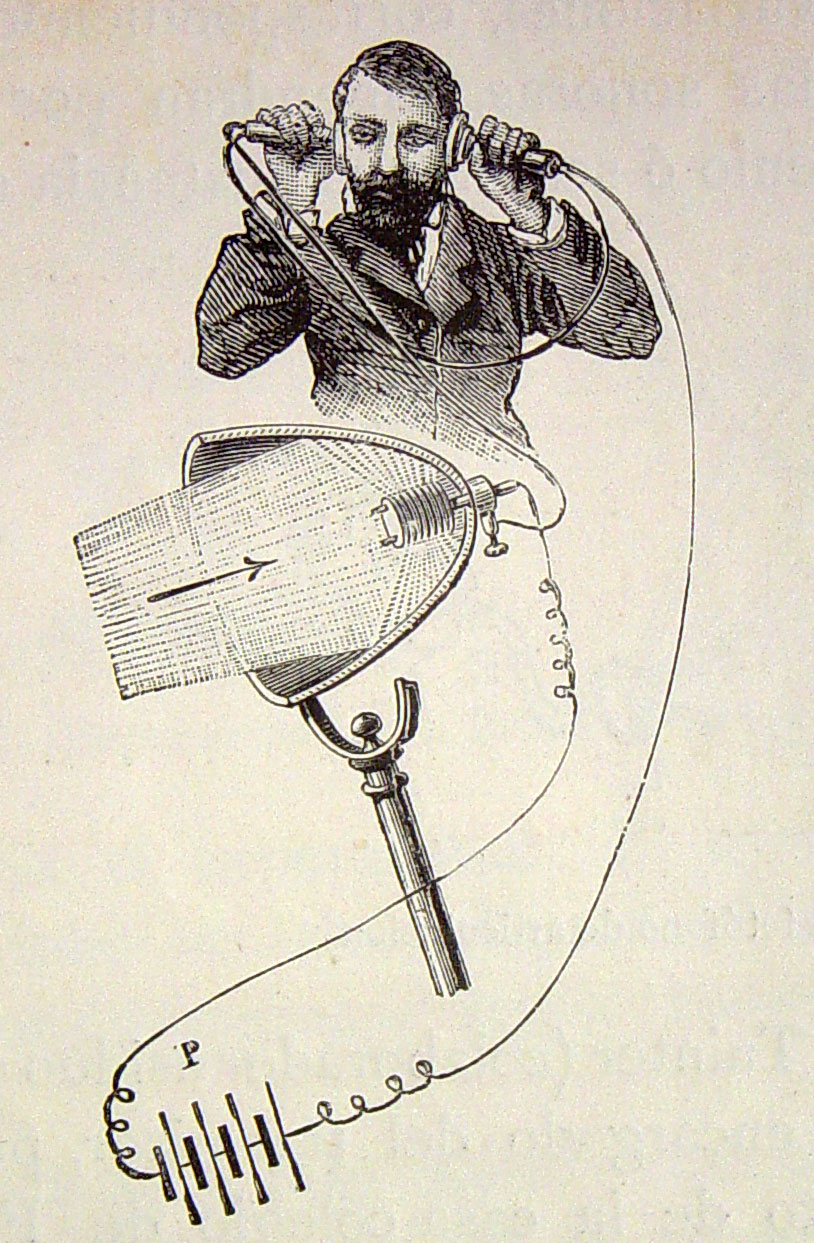
\includegraphics[angle=0,width=\textwidth]{./Figures/Photophone_receiver.jpg}
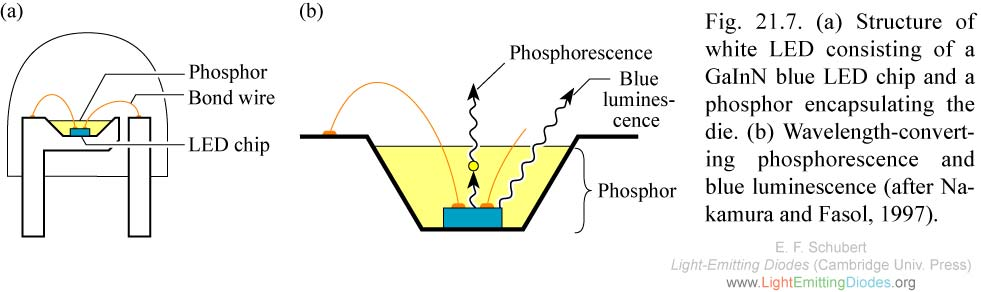
\includegraphics[angle=0,width=\figwidth]{./Figures/slide0011_image007.jpg}
\caption[Structure of a phosphorescence white LED]{Structure of a GaInN phosphorescence based White LED \cite{ledStructure}}%: Image courtesy of E.F Schubert, Cambridge Univ Press, www.LightEmittingDiodes.org }
%\floatfoot{Source: \url{http://www.ecse.rpi.edu/~schubert/Light-Emitting-Diodes-dot-org/chap21/F21-07 Nichia wh LED structu.jpg}}
 \label{fig:phosphor_led}
\end{figure}


The second technology fabricates three devices on a single chip. These devices produce three different colours that are combined to produce white light \ref{fig:RGB_led}. This is the more expensive technology but provides more flexibility in system design. The device has faster switching characteristics than phosphor based LEDs \cite{le2008high} as no second excitation is involved. These devices are also available in packages that have the control pins for the three different colours coming out of the case. These pins can be used to override three different information signals on three available colour wavelengths in a visible light communication scenario. In this way three fold data rate is achieved from a single device using Wavelength Division Multiplexing (WDM). Colour filters are used at the receiver end to separate wavelength multiplexed data streams from original white light.

\begin{figure}[hbtp]
\centering
%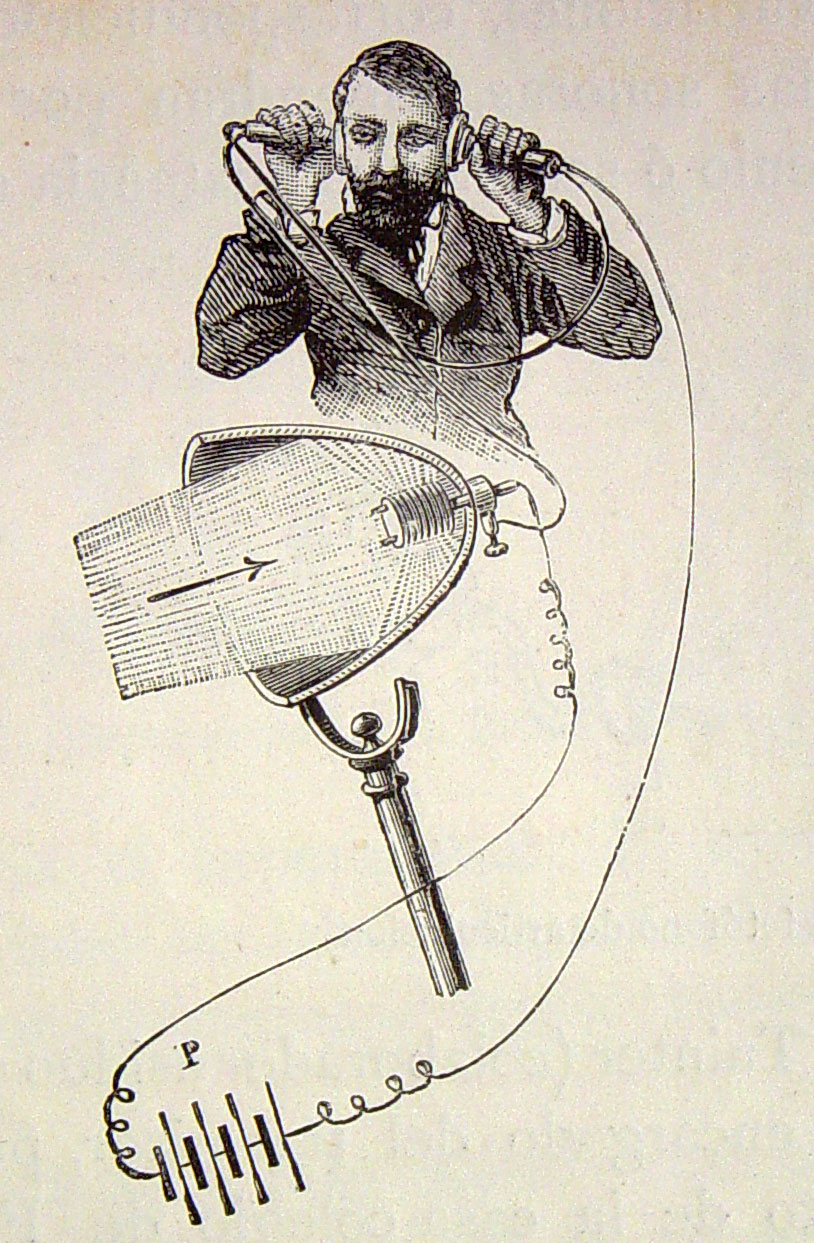
\includegraphics[angle=0,width=\textwidth]{./Figures/Photophone_receiver.jpg}
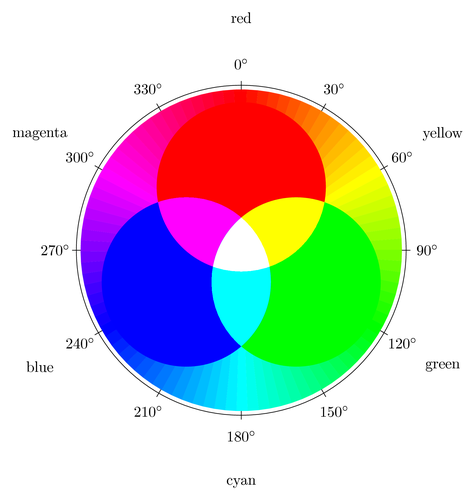
\includegraphics[angle=0,width=.5\textwidth]{./Figures/slide0018_image011.png}
\caption[White light from RGB colours]{White light from intermixing of different wavelengths in an RGB LED \cite{RGBlight}}
%\floatfoot{Source:\url{}}
%\floatfoot{Source: \url{http://media.texample.net/tikz/examples/PNG/rgb-color-mixing.png}}
\label{fig:RGB_led}



%\protect\footnote{and protect my footnotes}
\end{figure}

\section{Visible Light Communication Vs Infrared And Radio Transmission}
Visible light LED based data hotspots have many interesting advantages over other wireless networking technologies such as radio-frequency  and infrared transmission.

\begin{list}{$\ast$}{}
\item Radio spectrum used for wireless communication is getting close to saturation. It is estimated that the consumer bandwidth requirements double every year whereas the technology capacity doubles only in ten years.  Therefore experts are looking for alternate means to fill in this gap. VLC offers a promising new wireless technology with huge bandwidth.

\item Radio spectrum is largely regulated and it is costly to purchase bandwidth. VLC is free from such regulations and therefore it can be readily deployed.

\item There are certain health problems related with high power RF signals \cite{szmigielski1982accelerated} \cite{agarwal2009effects} \cite{wdowiak2007evaluation}. Living cells can be damaged when exposed to power signals for longer time. However there are no such issue with visible light communication.

\item Radio signals interfere with other electronics equipment causing malfunctioning of sensitive devices \cite{robinson1997interference} \cite{van2008electromagnetic}. VLC does not pose such problems which makes it a suitable candidate for access technology in hospital and air planes. 

\item RF equipment is costly and requires extra fixtures for devices. In contrast to that VLC uses the light source for data transmission. Driving the visible light source at high powers is much cheaper. Most of the mobile phones carry flash lights and cameras that have potential to be used as VLC transmitter and receiver respectively. It makes technology adoption at lower cost.

\item It is difficult to confine RF signals within the desired area and faces security risks from eavesdroppers.\cite{racherla2000security}. However visible light is highly directional that reduces the fear of signal capture by wrong recipients. Moreover opaque objects help confine the signal within a closed space. It is an appreciated feature of VLC for security and data privacy.

\item Visible light communication offers superiority over other optical data access technologies like infra-red and ultraviolet transmission. Though in principle it is not different from them, but being visible to eye it fulfils illumination requirements in addition to wireless communication.

\item Because infrared light is invisible, at high power levels it can damage the human eye without being noticed. In VLC's case, human eye closes by reflex action when it senses high powered illumination. That makes the later technology a safer option.

\item Though infrared and ultraviolet lights are directional too, it is somewhat difficult to align the transmitter and receiver because of invisibility of the signal stream. VLC is superior as the illumination can easily be directed to the point where it is required.

\item The information access cum illumination spot can easily be detected by naked eye. This is useful in public data access services. User can spot the places with stronger signal reception. For a comparison this convenience is not available in Wi-Fi systems.


\item Optical transmission is highly directional and needs line of sight signals for effective communication. Here radio transmission wins over VLC.

\item Visible light experiences higher attenuation in atmosphere. Therefore its range is shorter than IR and RF communication.

\end{list}

\section{Where VLC Is Used?}
 LED lights can be designed either to form a focused or a diffused light beam. Former configuration has found applications in point to point communication links.  The focused beam applications include free space optical (FSO) line-of-sight links and optical fibre communication. Though the communication may take place in visible light spectrum in above mentioned technologies, these are not categorized under visible light communication. VLC applies to the scenarios where transmitting light source is not a spacial communication device but rather its primary function is something else, like illumination \cite{komine2004fundamental} or signalling. This thesis focuses on applications where illumination is the main feature of LED light source and it provides ubiquitous communication as an added luxury \cite{VLCC}.

The VLC lights can be deployed indoors or outdoors with pros and cons of each scenario. In indoor environment, receiver gets light not only from direct light of sight but also from secondary reflections by room walls and other objects. In this case it is not all too necessary for transmitter and receiver to be in line of sight. However in outdoor situations this advantage may not exist.

\begin{figure}[hbtp]
\centering
%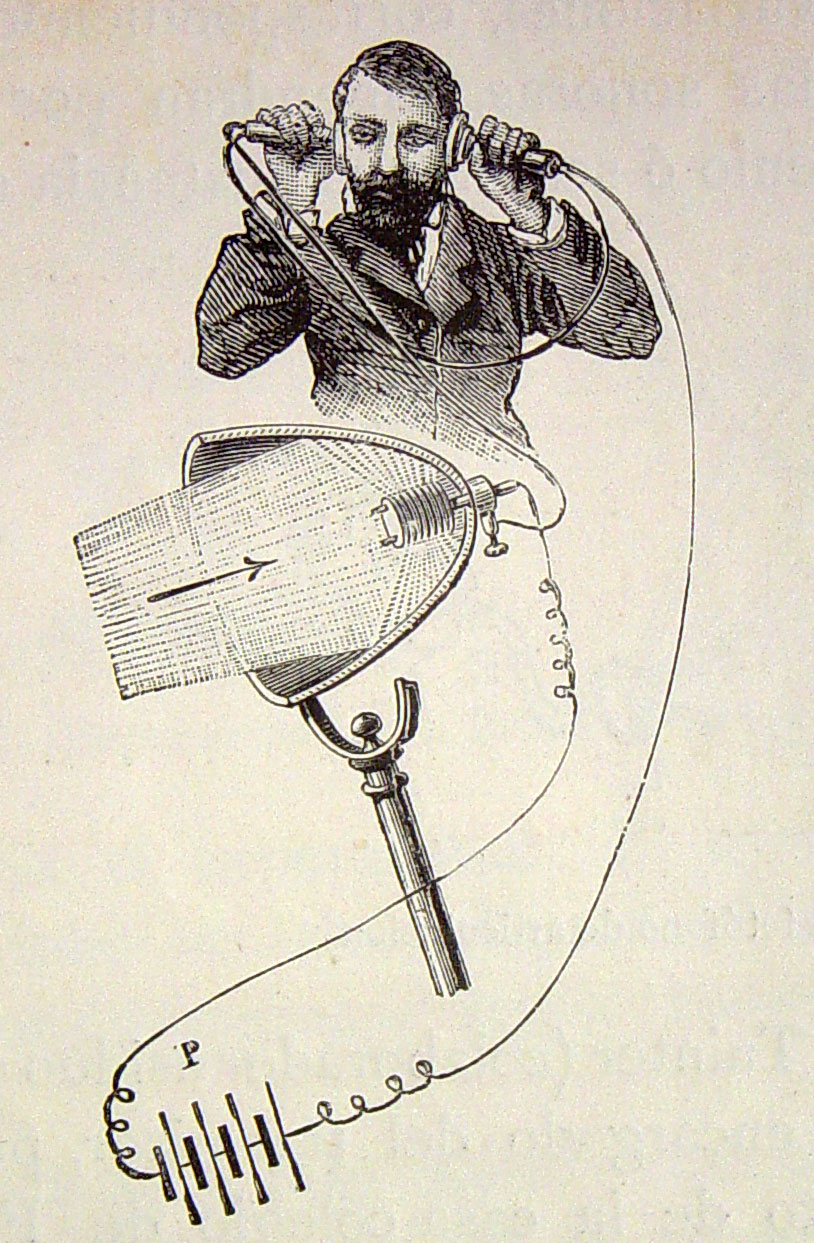
\includegraphics[angle=0,width=\textwidth]{./Figures/Photophone_receiver.jpg}
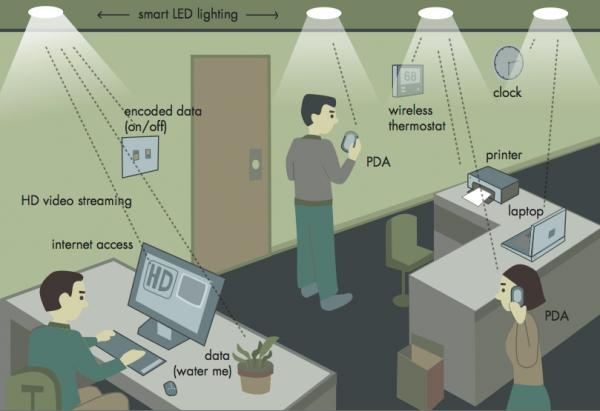
\includegraphics[angle=0,width=.9\textwidth]{./Figures/VLC_Room.jpg}

\caption[Visible light communication in office]{Visible light communication indoor scenario \cite{VLCroom}}
%\floatfoot{Source:\url{	www.eetimes.com/electronics-news/4199568/Visible-light-illuminates-a-new-approach-for-wireless-comms}}
 \label{fig:VLC_room}
\end{figure}

%Photographer's or artist's name (often not given)
%Name of subject or title of picture
%Date of picture (often not given)
%Title of website
%URL
%Date you accessed the picture.

The signals reflected by walls and other objects in indoor environment pose greater intersymbol interference due to multiple delayed versions of the same signal \cite{komine2004fundamental}. It puts a limit on maximum transmission speed. However outdoor lights do not suffer from this limitation. On the other hand outdoor lighting are affected by environmental conditions such as fog, smoke and rapid temperature variations. In indoor environment these conditions are very much under control.

In indoor environment, the positioning systems such as GPS largely fail or provide false reading due to inadequate RF signals \cite{dedes2005indoor}. In one of the VLC applications, light fixture sends information pulses with source position tags. A hand-held receiver device reads these tags from different light sources to estimate its position \cite{tanaka2009new}. This application is useful for sight impaired patients, helping them in navigation through hospitals corridors.

In departmental stores VLC light fixtures can be used to inform customers about different products in their vicinity. A cheap photo sensor mounted on the trolley receives this information and displays it on a small attached LCD screen. Similarly museums can use light sources placed to illuminate objects as well as transmit information about them. A tourist with a cheap hand held device pointed at illuminating LED can hear or read the information he wants without disturbing others. Even mobile phones can be used as the receiving device as cameras can be found on majority of the phones now a days.

A new term Li-Fi has been evolved to describe the wireless networking environment based upon visible light communication, inspired from Wi-Fi. There is research going on for embedding the power line communication (PLC) with VLC for ubiquitous broadband access networked computing \cite{komine2003integrated}.

Another form of VLC is proposed for vehicle to vehicle communication \cite{dunning2004inter}. The tail light of a car ahead communicates with the photosensor mounted on the car following behind. It has potential use as a collision avoidance technology. Another research focuses on data transmission by LED traffic signals to the surrounding vehicles \cite{arai2007experimental} about congestions warnings, alternate routes etc. It may also be possible to get map information from these signals.

Electronic sign boards can also be enabled to transmit data by modulating the light \cite{park2007information}. Similarly television sets, computer screens and back lights of mobile phone displays have been demonstrated to transmit information in the form of visible light. VLC has also found applications in high speed communication in underwater environment where radio signals undergo higher attenuation.
%------------------------ 

To summarize, white LED based lighting cum data transmission solutions can widely be used in home automation, broadcasting at shopping malls, precision indoor positioning and navigational aids, indoor wireless networks in hospitals, aircrafts and spaceships etc.

\section{Thesis Objectives}
The main objective of this thesis is to solve an important problem associated with the drive signal for information carrying light source. Dimming control of the communicating LED lights is an important requirement as lighting is their primary feature. However the information modulation and dimming control signals interfere with each other. Conventionally dual modulation techniques are used to mitigate this interference. We propose a novel line coding scheme, Variable Rate Multipulse Pulse Position Modulation (VR-MPPM), that achieves brightness control as well as data transmission using single modulation signal.

Power spectral density of the proposed encoding scheme is obtained to evaluate the effect of brightness level and brightness resolution on spectral characteristics. The underlying tradeoffs between brightness resolution and successful data transmission rate are evaluated for optimal performance. The proposed scheme is tested on FPGA based hardware setup to evaluate bit error performance at different brightness levels and brightness resolutions.

\section{Research Papers}
As part of this research, a conference paper \cite{siddique2011joint} was submitted to \emph{CCNC'2011 - Smart Spaces and Personal Area Networks}. The paper proposed the VR-MPPM line coding scheme for joint brightness control and data transmission of VLC lights. It presented simple iterative data encoding and decoding algorithms along with practical and numerical evaluation of the proposed scheme.

Another paper has been submitted to \emph{IEEE communications Letters} that analyses the spectral properties of VR-MPPM encoding schemes. The underlying tradeoffs between brightness resolution and symbol error rate are discussed to select optimal symbol frame size.

\section{Organization Of The Thesis}
In order to provide the theoretical background for the research work done in this thesis, the study of existing modulation schemes for joint dimming control and data communication of LED lamps is presented in chapter 2. In Chapter 3 the proposed modulation scheme is developed to jointly achieve brightness control and data transmission for a VLC light source. Simple iterative encoder and decoder algorithms are also developed that are explained with the help of simple examples. Chapter 4 evaluates the spectral properties of the proposed scheme. The spectrum analysis methodology is explained with the help of an example. The effect of symbol frame size and brightness level on power spectrum are evaluated. In Chapter 5, objective function for optimal selection of frame size for minimum symbol error rate and maximum brightness resolution is evaluated. Hardware implementation of the proposed line codes and dependence of symbol error rate on brightness index is  also observed in this part. Finally we draw our conclusions in Chapter 6.

%\section{Research Papers}
%As part of this research, a conference paper \cite{siddique2011joint} has been presented in \emph{CCNC'2011 - Smart Spaces and Personal Area Networks}. The paper proposed the VR-MPPM symbol encoding algorithm along with its practical and numerical evaluations.


%\textbf{Joint Brightness Control and Data Transmission for Visible Light communication Systems based on White LEDs}
%We have submitted another paper to \emph{IEEE communications Letters} that analyses the spectral properties of VR-MPPM encoding schemes. The underlying tradeoffs between brightness resolution and symbol error rate for selection of optimal symbol frame size are also discussed.